\section[Cycle de vie]{Cycle de vie d'une application}
\subsection{Définition}
\begin{frame}{\subsecname}
	\begin{block}{}
		Ensemble d'étapes intervenant au cours du développement d'un projet informatique
	\end{block}
	\todo{définition rapido à partir du mémoire pour rafraîchir les mémoires}
\end{frame}

\subsection{Cas de la Nouvelle-Aquitaine}

\begin{frame}{Le projet}
	\begin{block}{Des portails web}
		\note{Pour décrire les différents services et aides offerte par la région. Chacun s'adresse à un public différent}
		\begin{itemize}
			\item Transport
			\item Guide des aides
			\item Portail Jeunes
			\item Régie d'Information
			\item Entreprise
			\item ...
		\end{itemize}
	\end{block}
\end{frame}

\begin{frame}{Illustration}
	\begin{center}
		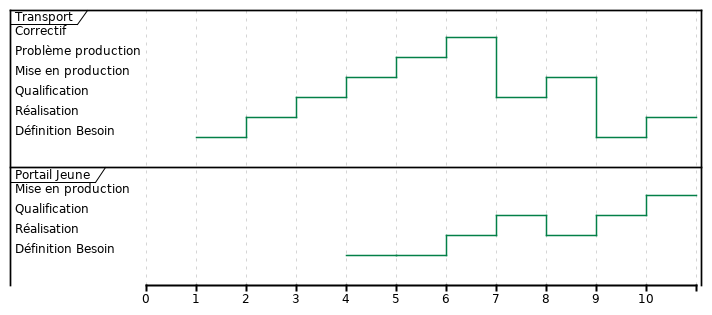
\includegraphics[width=0.80\textwidth]{../img/cycle-vie-naq.png}
	\end{center}
	\todo{Frames manquantes pour détailler le cycle de vie}
\end{frame}